% This must be in the first 5 lines to tell arXiv to use pdfLaTeX, which is strongly recommended.
\pdfoutput=1
% In particular, the hyperref package requires pdfLaTeX in order to break URLs across lines.

\documentclass[11pt]{article}

% Remove the "review" option to generate the final version.
% \usepackage[review]{acl}
\usepackage{acl}

\usepackage{todonotes}
\newcommand{\todoinari}[2][]{\todo[color=red!40,#1]{Inari: #2}}
\newcommand{\todoregina}[2][]{\todo[color=red!40,#1]{Regina: #2}}

\def\scasp{s(CASP) }

% for strikeout
\usepackage[normalem]{ulem}

% table width
\usepackage{tabularx}

% colour
\definecolor{dimgray}{rgb}{0.1, 0.1, 0.21}
%\definecolor{dimgray}{rgb}{0.33, 0.33, 0.33}

% Standard package includes
\usepackage{times}
\usepackage{latexsym}

% For proper rendering and hyphenation of words containing Latin characters (including in bib files)
\usepackage[T1]{fontenc}
% For Vietnamese characters
% \usepackage[T5]{fontenc}
% See https://www.latex-project.org/help/documentation/encguide.pdf for other character sets
% This assumes your files are encoded as UTF8
\usepackage[utf8]{inputenc}

% This is not strictly necessary, and may be commented out,
% but it will improve the layout of the manuscript,
% and will typically save some space.
\usepackage{microtype}

% to override enumerating symbol
\usepackage{enumitem}

\usepackage{graphicx}
\usepackage{ifxetex,ifluatex}
\usepackage{fixltx2e} % provides \textsubscript
% use upquote if available, for straight quotes in verbatim environments
\IfFileExists{upquote.sty}{\usepackage{upquote}}{}
\ifnum 0\ifxetex 1\fi\ifluatex 1\fi=0 % if pdftex
  \usepackage[utf8]{inputenc}
\else % if luatex or xelatex
  \ifxetex
    \usepackage{mathspec}
    \usepackage{xltxtra,xunicode}
  \else
    \usepackage{fontspec}
  \fi
  \defaultfontfeatures{Mapping=tex-text,Scale=MatchLowercase}
  \newcommand{\euro}{€}
\fi
% use microtype if available
\IfFileExists{microtype.sty}{\usepackage{microtype}}{}
\usepackage{color}
\usepackage{fancyvrb}
\newcommand{\VerbBar}{|}
%\newcommand{\VERB}{\Verb[commandchars=\\\{\}]}
\newcommand{\VERB}{\Verb[commandchars=\\\{\},codes={\catcode`$=3\catcode`_=8}]}
\DefineVerbatimEnvironment{HighlightingFancy}{Verbatim}{commandchars=\\\{\},codes={\catcode`$=3\catcode`_=8}}
\DefineVerbatimEnvironment{Highlighting}{Verbatim}{commandchars=\\\{\}}

% Add ',fontsize=\small' for more characters per line
\usepackage{framed}
\definecolor{shadecolor}{RGB}{248,248,248}
\newenvironment{Shaded}{\begin{snugshade}}{\end{snugshade}}
\newenvironment{EmptyItem}{\begin{itemize} \item[]}{\end{itemize}}
\newcommand{\KeywordTok}[1]{\textcolor[rgb]{0.13,0.29,0.53}{\textbf{{#1}}}}
\newcommand{\DataTypeTok}[1]{\textcolor[rgb]{0.13,0.29,0.53}{{#1}}}
\newcommand{\DecValTok}[1]{\textcolor[rgb]{0.00,0.00,0.81}{{#1}}}
\newcommand{\BaseNTok}[1]{\textcolor[rgb]{0.00,0.00,0.81}{{#1}}}
\newcommand{\FloatTok}[1]{\textcolor[rgb]{0.00,0.00,0.81}{{#1}}}
\newcommand{\CharTok}[1]{\textcolor[rgb]{0.31,0.60,0.02}{{#1}}}
\newcommand{\StringTok}[1]{\textcolor[rgb]{0.31,0.60,0.02}{{#1}}}
\newcommand{\CommentTok}[1]{\textcolor[rgb]{0.56,0.35,0.01}{\textit{{#1}}}}
\newcommand{\OtherTok}[1]{\textcolor[rgb]{0.56,0.35,0.01}{{#1}}}
%\newcommand{\AlertTok}{1}{\textcolor[rgb]{0.94,0.16,0.16}{{#1}}}
\newcommand{\AlertTok}[1]{\textcolor[rgb]{0.74,0.01,0.01}{{#1}}}
\newcommand{\FunctionTok}[1]{\textcolor[rgb]{0.00,0.00,0.00}{{#1}}}
\newcommand{\RegionMarkerTok}[1]{{#1}}
\newcommand{\ErrorTok}[1]{\textbf{{\color{gray}#1}}}
\newcommand{\NormalTok}[1]{{#1}}

\graphicspath{ {./images/} }
% If the title and author information does not fit in the area allocated, uncomment the following
%
%\setlength\titlebox{<dim>}
%
% and set <dim> to something 5cm or larger.

%Set the title and author using \verb|\title| and \verb|\author|. Within the author list, format multiple authors using \verb|\and| and \verb|\And| and \verb|\AND|; please see the \LaTeX{} source for examples.

%By default, the box containing the title and author names is set to the minimum of 5 cm. If you need more space, include the following in the preamble:
%\begin{quote}
%\begin{verbatim}
%\setlength\titlebox{<dim>}
%\end{verbatim}
%\end{quote}
%where \verb|<dim>| is replaced with a length. Do not set this length smaller than 5 cm.



\title{Towards CNL-based verbalization of computational contracts}


% Author information can be set in various styles:
% For several authors from the same institution:
% \author{Inari Listenmaa \and Maryam Hanafiah \and Nur Liyana Binte Abdul Muthalib \and Regina Cheong \and Andreas Källberg \\
% \author{Inari Listenmaa \and Maryam Hanafiah \and Liyana Muthalib \and Regina Cheong \and Andreas Källberg \\

% if the names do not fit well on one line use
         \author{Inari Listenmaa \\ {\bf Maryam Hanafiah} \\ {\bf Regina Cheong} \\ {\bf Andreas Källberg} \\
        \texttt{\{ilistenmaa,  maryammh, reginacheong, akallberg\}@smu.edu.sg} \\
         Singapore Management University}

% For authors from different institutions:
% \author{Author 1 \\ Address line \\  ... \\ Address line
%         \And  ... \And
%         Author n \\ Address line \\ ... \\ Address line}
% To start a seperate ``row'' of authors use \AND, as in
% \author{Author 1 \\ Address line \\  ... \\ Address line
%         \AND
%         Author 2 \\ Address line \\ ... \\ Address line \And
%         Author 3 \\ Address line \\ ... \\ Address line}

%\author{Inari Listenmaa \\
%  Singapore Management University / Address line 1 \\
%  \texttt{ilistenmaa@smu.edu.sg} \\\And
%  Second Author \\
%  Affiliation / Address line 1 \\
%  \texttt{email@domain} \\}

\begin{document}
\maketitle

\begin{abstract}
We present a CNL, which is a component of L4, 
a domain-specific programming language for drafting laws and contracts.
Along with formal verification, L4's core functionalities include natural language generation.
We present the NLG pipeline and an interactive process for ambiguity resolution. 

\end{abstract}

\section{Introduction}
\label{sec:intro}
% \todo{RC: I am not sure where to put the current legal systems n motivation section 1.1 and 1.2 which reviewers ask for motivation n current gaps}
We introduce L4, a prototype\footnote{L4 is a work in progress, and this article presents a snapshot of the project as of June 2021. Any concrete examples of L4 code or the CNL may change in a few months.} 
domain-specific language (DSL) for drafting laws and contracts. 
%L4 draws its theoretical foundations from prior art in defeasible, default, and modal logics as applied to legal reasoning \cite{governatori_variants_2007}, and further builds on existing legal formalisms such as LegalRuleML~\cite{palmirani2011legalruleml}, FormaLex~\cite{gorin_software_2011}, POETS CSL~\cite{andersen_domain-specific_2014} and Catala~\cite{merigoux2021catala}.
L4's applied focus places it within the ``Rules as Code'' movement (e.g. \citet{openfisca_openfisca_nodate}, Catala~\cite{merigoux2021catala}) that itself draws on early computational law thinking \cite{sergot_british_1986, love_computational_2005}. But rather than focusing on encoding laws into existing programming languages, we devise an external DSL designed for legal specification. From this specification, we generate a range of output formats. 
%the interpreter supports inter-operability with an ecosystem of third-party tools. 
Key augmentations include IDE support, formal verification engines, transpilation to operational rule engines, and natural language generation (NLG). 
The latter is done via a CNL implemented in Grammatical Framework (GF, \citeauthor{ranta_grammatical_2004} \citeyear{ranta_grammatical_2004}), and will be the focus of this paper.

\paragraph{Motivation for a DSL}
The intended user of L4 is not a law firm, but rather an organization or a person who wants to bypass law firms. 
As a possible early adopter profile, we envision a technology startup drafting their initial agreements in L4. Drafting rules as code enables the owners to keep track of dependencies and detect potential conflicts, without needing a lawyer.

More generally, a formal encoding of rules allows the creation of different end-user applications. When the specification changes, it is only necessary to implement the change in the L4 source, and regenerate the applications.

\paragraph{Motivation for NLG}
In order to communicate with the rest of the world, the L4 encoding needs to be translated into non-technical end-user products, such as natural language documents and interactive web applications.
%formal verification, diagram visualization and natural language---
We present two NLG applications in this paper.

\begin{itemize}
    \item An expert system, which generates interview questions from L4 code, uses the user input to query an automated reasoner, and presents the reasoner's answers in natural language (Section~\ref{sec:expert_system}).
    \item In the future we aim to support the generation of an isomorphic natural language version of L4 code (Section~\ref{sec:NLrep}).
    %\item Generate natural language feedback from automated reasoners and formal verification engines (Section~\ref{sec:SCASPans}).
    %\item Perform automated reasoning on L4 code, and generate natural language answers 
\end{itemize}

In the remainder of the paper, we present a small example of L4 code in Section~\ref{sec:example}, 
a brief introduction to the NLG pipeline in Section~\ref{sec:nlg}, 
the CNL in Sections~\ref{sec:cnl} and \ref{sec:parsing}, 
and finally, future work in Section~\ref{sec:futurework}.

%\subsection{Current legal system}
%\label{sec:motivation}
%At a high level, the typical process for filing a case may be summarized more or less as the following (\citeauthor{civil_lawsuit_process}): \todo{its url in ref is overflowing the margin. need help}
%https://www.hopkinsroden.com/news-and-resources/posts/2019/december/the-civil-lawsuit-process-from-start-to-finish/
%\begin{itemize}
%    \item Consulting an attorney. 
%    \item Filing the complaint to the court and duplicating a copy to the defendant for his refute or counter-claim.
%    \item A trial process in the hearing of a court.
%    \item Verdict delivery by the judge or jury.
%    \item Filing an appeal should a party disagree with the verdict.
%\end{itemize}
%This lengthy process often incurs many days, if not weeks or months for complex cases, and saps many resources. If there is a formula to estimate the duration and cost, it would most definitely be directly proportional, possibly even exponentially-correlated to the number of parties, number of steps and number of charges involved. 

%\subsection{Motivation}
%The motivation for developing L4 and hence, the underlying CNL, aims to address this gap in the legal system. It seeks to economise and streamline the process by achieving the following goals:
%\begin{itemize}
%    \item Empower a non-legally-trained person. 
%    \item Support the legal and contract drafting process. 
%    \item Expedite the file-to-verdict process.
%\end{itemize}
%The isomorphic natural language of L4 codes and natural language feedback from automated reasoners aid the draftsmen by presenting the interpretation of the law and contractual terms. This supports the refinement of the drafting process ensuring alignment with intent is achieved.
%The interview process and natural language feedback provide transparency for the layman regarding his/her legal obligations.

%The product is thus a systematic approach, without bias, for an objective conclusion. Different approaches (i.e. justifications models) to arrive at a similar conclusion could also be displayed, further enhancing the drafting process. 
%These accessibility and transparency benefits help streamline and expedite the typical application, submission, processing and eventual communication of conclusion. 

%reference to jason's blogpost and do-not-pay
% https://medium.com/computational-law-diary/introducing-l4-docassemble-69ce4b1fb1e7
% https://techcrunch.com/2020/12/10/robot-lawyer-startup-donotpay-now-lets-you-file-foia-requests/#:~:text=DoNotPay%2C%20the%20consumer%20advice%20company,sue%20companies%20for%20small%20claims.

%In addition, we present IDE support for resolving syntactic ambiguities, using GF's Resource Grammar Library with custom extensions to parse user input, and transform it into questions about the syntactic structure (Section~\ref{sec:lexicon}).

%We envision the final form to resemble more SQL and less first-order logic.


\begin{figure}[t]
\begin{Shaded}
\begin{Highlighting}[]
\CommentTok{\# types and predicates}
\KeywordTok{class}
  Business
  LegalPractitioner

\KeywordTok{decl}
  MayAcceptAppointment 
    \KeywordTok{:} LegalPractitioner -> 
      Business -> Bool
  UnauthorizedSharingFees
    \KeywordTok{:} Business -> Bool
    
\CommentTok{\# rules}
\KeywordTok{rule} \AlertTok{<no_sharing_fees>}
\KeywordTok{ for} \NormalTok{b} \KeywordTok{:} Business,
     \NormalTok{l} \KeywordTok{:} LegalPractitioner
\KeywordTok{  if} \NormalTok{UnauthorizedSharingFees b}
\KeywordTok{then not} \NormalTok{MayAcceptAppointment l b}
\end{Highlighting}
\end{Shaded}
\caption{L4 code for a rule "legal practitioner may not accept an appointment in a business that involves sharing fees with unauthorized persons"}
\label{fig:minimalL4code}
\end{figure}


\section{L4 example}
\label{sec:example}
We demonstrate L4 with the following scenario, simplified from an experiment to draft existing regulations in L4 \cite{morris2021rule34}.
There are certain rules for whether a legal practitioner may accept an appointment in a business. 
For instance, if the business would share the legal practitioner's fees with unauthorized persons, the legal practitioner is not allowed to accept the appointment.




In Figure~\ref{fig:minimalL4code}, we model this rule in L4 (in its current syntax).
First, we declare the data types for {\small \texttt{Business}} and {\small \texttt{LegalPractitioner}}, and two predicates, {\small \texttt{MayAcceptAppointment}} and {\small \texttt{UnauthorizedSharingFees}}. 
Then, we formulate a rule to say that a legal practitioner may not accept an appointment in a business which involves sharing fees with unauthorized persons. The current syntax of L4 is adopted from functional programming languages.
For example, the type signature for {\small \texttt{F : A~$\rightarrow$~B $\rightarrow$ Bool}} means \textit{``the function F takes an A and a B, and returns a Boolean''}.

%We are using the following piece of L4 code as a running example. 
%The following is a minimal piece of L4 code in its current syntax. First, we declare a datatype for \texttt{Person}, and two predicates, \texttt{Jaywalk} and \texttt{Criminal}. Then, we formulate a rule to say that jaywalking is criminal.
%the unauthorized sharing of fees is prohibited.
%\todo{Replace the whole example with something from Section 34.}


%Already this simple example presents challenges for NLG. 
%As a naive solution, we can look up the names of the classes and predicates from any large lexicon. %the GF-WordNet lexicon \cite{angelov2020parallel}. 
%In case of more complex predicate names, like \texttt{DerogatesFromDignityOfLegalProfession}, we can split them into words and parse. 
%In most such resources, \textit{unauthorized} would be unambiguously listed as an adjective,
%but \textit{prohibited} could be an adjective or a verb: we need to know whether to generate \textit{these businesses are prohibited} or \textit{the law prohibited these businesses}.
%We need to know the part of speech for every predicate,

In the simplest case, we can look up the names of the classes and predicates from any large lexicon: 
{\small \texttt{Business}} is just a single noun, 
and {\small \texttt{LegalPractitioner}} is either a compositional noun phrase of \textit{legal} (adjective) and  \textit{practitioner} (noun), or a multi-word expression in a domain-specific lexicon. %would ideally match a pre-existing multiword token, but  when split, matches an adjective and a noun, or a multiword
The two predicates are more complex, since they involve a full verb phrase. Figure~\ref{fig:optionalLexicon} shows  an optional lexicon, where the user can write a CNL description of the predicates. 


A predicate name like {\small \texttt{UnauthorizedSharing- Fees}} is used throughout the program code, and the NLG engine will use the description \textit{involves sharing fees with unauthorized persons}---not as an immutable string, but parsed with a GF grammar
into a deep syntax tree. 
The placeholders, shown in the description of {\small \texttt{MayAcceptAppointment}}, are optional, if the arguments appear predictably: subject for a unary predicate, and subject and object for a binary predicate. Any CNL description of the form \textit{predicate} is treated as \textit{{\small \texttt{\{Arg1\}} } predicate {\small \texttt{\{Arg2\}}}}.
However, if we wanted to have an argument in another role, then the placeholders are obligatory, as shown in Figure~\ref{fig:unauthorizedSharingFees}. 
%In the remainder of the paper, we will use the version from Figure~\ref{fig:optionalLexicon}, because it is simpler.



\begin{figure}[t]
\begin{Shaded}
\begin{Highlighting}[]
\CommentTok{# optional CNL descriptions}
\KeywordTok{lexicon}
  UnauthorizedSharingFees 
   \KeywordTok{@} \StringTok{"involves sharing fees with}
     \StringTok{ unauthorized persons"}
  MayAcceptAppointment 
   \KeywordTok{@} \StringTok{"\{LegalPractitioner\} may}
     \StringTok{ accept an appointment}
     \StringTok{ in \{Business\}"}
\end{Highlighting}
\end{Shaded}
\caption{Optional lexicon with CNL description of predicates}
\label{fig:optionalLexicon}
\end{figure}

\begin{figure}[b]

\begin{Shaded}
\begin{Highlighting}[]
\KeywordTok{decl}
  UnauthorizedSharingFees 
   \KeywordTok{:} Business
     -> LegalPractitioner 
     -> Bool
   \KeywordTok{@} \StringTok{"\{Business\} involves sharing}
     \StringTok{ \{LegalPractitioner\}'s fees} 
     \StringTok{ with unauthorized persons"}
\end{Highlighting}
\end{Shaded}
\caption{Alternative example, where UnauthorizedSharingFees is a binary predicate}
\label{fig:unauthorizedSharingFees}
\end{figure}

%We present the CNL in more detail in Sections~\ref{sec:cnl}~and~\ref{sec:parsing}.

%For multilingual applications, we also need to know which sense of \textit{person} to use: human being or grammatical category (as in "3rd person singular"). That's future work but it will use WordNet glosses.

\section{NLG from L4}
\label{sec:nlg}


L4 is implemented using Alex \cite{dornan2003alex} and Happy \cite{marlow1997happy}. 

First, an L4 program is parsed into an L4 abstract syntax tree (AST). That tree is used as an input to all of the output formats named in Section~\ref{sec:intro}. 
The L4 abstract syntax and the CNL descriptions are used in two NLG applications, which are presented in the remainder of this section.

%The natural language generation also uses the CNL descriptions, which are parsed with a GF grammar. 
%This loosely overlaps with the micro-planning phase in a standard NLG pipeline. L4 includes a lexicon which is defined by the user or derived from the predicates, and aggregation occurs when the L4 rules are parsed into GF.
\subsection{Expert system}
\label{sec:expert_system}


\citet{listenmaa2021inlg} presents the expert system in more detail. In this paper, we only introduce what is necessary to set the context for the CNL.


\paragraph{Interview questions}
\label{sec:DAinterview}

The first output target for the expert system is a set of interview questions. Suppose we want to ask a user interactively whether their business may employ a legal practitioner: then we transform every predicate that is a precondition to {\small \texttt{MayAcceptAppointment}} into a question.

\begin{quote}
\begin{enumerate}
\item Is your business incompatible with the dignity of the legal profession?
\item Does your business involve sharing fees with unauthorized persons?
\item \dots
\end{enumerate}
\end{quote}

The questions are embedded in a \citeauthor{docassemble} interview. Docassemble is an open-source legal expert system, where
users answer a set of questions through a browser interface. Their responses are then compiled together into a document, or processed further in other applications. In our system, we use the answers to query an automated reasoner.

%output which is either 
%\begin{itemize}
%    \item assembled documents in PDF, RTF or DOCX format which users can download or e-mail;
%    \item an application submission;
%    \item an API interaction; or
%    \item a redirection to other website resources.
%\end{itemize}

%\todoregina{explain a bit more about the interview and its purposes --- maybe ask Jason/Alfred for input. Also check out what to cite for Docassemble/other similar systems?}

\paragraph{Reasoner output in natural language}
\label{sec:SCASPans}

The second output target is a verbalization of answers that we get from an automated reasoner.
Previously we posed questions to the user---suppose they answered ``yes'' to question 2. The user input is sent to an automated reasoner, in order to query whether the user may employ a legal practitioner in their company. The reasoner's answer to the query is then rendered in natural language.

\begin{quote}
Your business may not employ a legal practitioner, because
\begin{itemize}
\item it involves sharing fees with unauthorized persons, and
\item a legal practitioner may not accept an appointment in a business that shares fees with unauthorized persons.
\end{itemize}
\end{quote}



The reasoner we use is \scasp \cite{arias2018constraint}: a logic programming language for Constraint Answer Set Programming.
%\cite{schwitter2012answer} p27 ???
%and can be used for reasoning and formal verification.
The parameters defined in an L4 source file are used for producing the Docassemble interview and \scasp code.
Using the user inputs to the interview questions to execute the \scasp code, a solution satisfying all the constraints is generated. 
The solution is then restructured in natural language and becomes the conclusion the user receives.

As the NLG process involves restructuring, this necessitates disambiguation at the input phase. For instance, the transformation of \textit{involves sharing fees} to \textit{a business that shares fees} is only possible if we know that \textit{sharing} is a gerund form of the verb \textit{share}, and not just a noun.
The disambiguation is discussed further in Section 5.    

Our work differs from approaches such as \citet{schwitter2012answer} in that we don't use CNL to formulate a specification or query---we use CNL as means to thoroughly understand the user predicates, so that we can verbalize answers. Our approach is more similar to \citet{devos2012annotating}, who annotate answer-set programs for verbalization, except that we are not limited to ASP.

%This verbalization into natural language best corresponds to the surface realization phase of the NLG pipeline. 
%---but in our system, it is only one of the output targets.

%Prior work on verbalising ASP answers includes \cite{erdem2011bioquery,erdem2015generating,schwitter2012answer,schwitter2013jobs,guy_schwitter2017peng,fang2017approach}.

%[ Future paper ]Use an example -- jaywalking or more complex
%\begin{itemize}
%\item Is there any person?
%\item What is the name of this person?
%\item Is there another person?
%\item What is the name of this person?
%\item (loop until all persons' names are input)
%\item Was there a road? 
%\item Was the road meant for motor vehicles?
%\item Did the person cross the road?
%\item Was there was a pedestrian traffic where the person crossed the road?
%\item Was the traffic light green when the person crossed the road?
%\end{itemize}
%In the above, the person is only a jaywalker when the person crossed a road meant for motor vehicles when the light was not green.

%\todoregina{Discuss with Inari}
%* We created a DA interview from a \scasp code and a LExSIS file generated from an L4 source file.

%* Then we ran the interview, got answers from user, translate the answers to \scasp code then send the query to the \scasp reasoner with the rules and facts described by the user

%* Then the conclusion in \scasp is finally verbalized  in natural language

%\todoregina{example of our output and how it works in the pipeline with Docassemble.}
%https://www.overleaf.com/project/6065b6dcbccbab4bf33d047b
 

\subsection{Isomorphic natural language representation}
\label{sec:NLrep}

Our future work includes an isomorphic representation of the L4 rules in a natural language as an output target. 
Suppose our previous rule about unauthorized fee sharing is just one rule among many that dictate whether or not a lawyer is allowed to accept an appointment.
Then the isomorphic representation would print out a comprehensive guide on employing legal practitioners---for instance, in a form of a contract to be signed, or as a set of regulations to be published on a web page. If the underlying rules change, then a new document can be generated from an updated L4 source.

On the level of individual rules, we follow \citeauthor{ranta2011translating}'s \citeyearpar{ranta2011translating} translation from logic to natural language:
the first step is a literal translation from the programming language abstract syntax to GF abstract syntax, 
followed by internal transformation of the GF trees to achieve more natural output.
%For example, \textit{there is a business B such that B is }
However, this work is only in the absolute beginning, and we haven't solved the difficult questions of generating a full NLG pipeline \cite{reiter_dale_2000} to output a complete document from the L4 code.

%Regardless the techniques used to produce the future document, it will need all the information



%legal businesses and the guide contains labels which activities are prohibited. 

%By executing the rule for \texttt{prohibited businesses}, we could output all prohibited activities in natural language, The output will be as follows.

%\begin{quote}
%The following business activities are prohibited:
%\begin{itemize}
%    \item sharing fees with unauthorized persons
%    \item activities incompatible with the dignity of the legal profession
%    \item \dots
%\end{itemize}    
%\end{quote}


\section{CNL}
\label{sec:cnl}

All of the NLG depends on correct understanding of whatever entities the user defines. Therefore we are using a CNL to restrict user input. %We saw a minimal example in Section~\ref{sec:example}, with the snippet ``is prohibited''. 
In this section, we explain the general principles of the design and implementation, and in Section~\ref{sec:parsing}, we explain how ambiguous user input is transformed into CNL variants, with concrete examples.


\subsection{Goal of the CNL}
Note that the CNL does {\bf not} have formal semantics---L4 as an actual programming language, with its formal verification and transpilation to operational engines, is better suited for that. 
The CNL is primarily a tool for getting a syntactically precise source for NLG.
The default mode of the NLG is a natural-looking, potentially imprecise language. But we envision an option to output syntactically precise CNL as well, if the user so wishes. %\footnote{Maybe it will prevent a lawsuit to use brackets for defining a scope of a modal verb.}


%The CNL is, instead, a source for potentially multilingual NLG. We rather transform the user's description into different communicative contexts (see Section~\ref{sec:nlg}), and in the future, into multiple languages. 
%We envision the default mode of the NLG to be a more natural

%We presented the current NLG scenarios in Section~\ref{sec:nlg}, and they all require a thorough understanding of the syntactic structures in order to produce fluent and grammatically correct text. 
%For a multilingual case, it is absolutely important to have the internal syntactic structures right, but even in a monolingual case, we retain the option to produce disambiguated output. 
%Rather trivial natural language ambiguities have resulted in lawsuits before, so it could be a useful feature to output a contract that makes explicit, say, scopes of modals, through brackets or a slightly unnatural word order.



\subsection{CNL design}
\label{sec:cnlDesign}
The CNL itself is a subset of English language, with disambiguation techniques à la Attempto Controlled English \cite{fuchs_attempto_1996}, ClearTalk \cite{skuce2003controlled} and other CNLs with an unambiguous syntax---see \citet{kuhn2014survey} for a survey. The current language features include
\begin{itemize}
    \item Hyphens for compound nouns: \textit{parking-fee}
    \item Brackets and word order to show attachment: \\ 
            \textit{[saw with a telescope] the astronomer} \\ 
            \textit{any [(business, trade or calling) in Bali]}
    \item Disambiguation for past tense. If the fragment has no disambiguating context, we assume: \\
            \textit{did prohibit} is past tense, \textit{prohibited} is past participle. 
\end{itemize}

Ambiguity between transitive and intransitive is resolved based on the arity of the predicate. Note that a predicate can be any part of speech, and any part of speech can be transitive or intransitive.
    %any part of speech can be transitive
    %Transitive form of verbs, adjectives, nouns are denoted by an arity of 2 e.g V2, A2, N2 respectively while intransitives are denoted by the arity of 1 which is not displayed by default. 
    Take a word like \textit{clear}, which can be a noun, verb or an adjective. If no CNL description is given, we assume the following:
    \begin{itemize}
         \item \texttt{\small Clear~:~X $\rightarrow$ Y $\rightarrow$ Bool} is a transitive~verb, \textit{X clears Y}, and
         \item \texttt{\small Clear~:~X $\rightarrow$ Bool} is an intransitive adjective, \textit{X is clear}. 
         
    \end{itemize}
         
\noindent If we want to use another part of speech or arity, we need to provide a CNL description.
    \begin{itemize}
        \item \texttt{\small Clear~:~X $\rightarrow$ Bool} \\ 
              \texttt{\small {\color{white}Clear~}@ "\{X\} clears"} \\      %   with the description \\ \textit{ \texttt{\small{[A]}} clears}
              is an intransitive verb (e.g. ``the clouds clear''),
        \item \texttt{\small Clear~:~X $\rightarrow$ Bool} \\ %is a noun with description {\it \texttt{\small[A]}} is in the clear}.
              \texttt{\small {\color{white}Clear~}@ "\{X\} is in the clear"} \\ is an adverbial where {\it clear} is a noun, and 
        \item \texttt{\small Clear~:~X $\rightarrow$ Y $\rightarrow$ Bool} \\ 
              \texttt{\small {\color{white}Clear~}@ "\{X\} is clear to \{Y\}"} \\      %   with the description \\ \textit{ \texttt{\small{[A]}} clears}
              is a transitive adjective, which takes its complement with the preposition {\it to}.
              

    \end{itemize}

% In general, the explanation below is not correct. You are confusing valency (transitive vs. intransitive) with predicative vs. attributive.


%         - transitive verb \texttt{\small  Clear~:~Person $\rightarrow$ Object $\rightarrow$ Bool} \textit{ e.g. I clear the mess } \\
%  ** Correct

%         - transitive adjective \texttt{\small Clear~:~A2 $\rightarrow$ N $\rightarrow$ Bool} \textit{e.g. clear (skies)} \\
%  ** Incorrect: clear is still intransitive, it's just in an attributive position here. Actually transitive adjective would be something like, "it is (clear to me)"

%         - intransitive verb \texttt{\small  Clear~:~N $\rightarrow$ V $\rightarrow$ Bool} \textit{e.g. (the clouds) clear } \\
%  ** Correct

%         - intransitive adjective \texttt{\small Clear~:~N $\rightarrow$ A $\rightarrow$ Bool} \textit{e.g. (the skies) are clear} \\
%  ** Incorrect explanation: clear is indeed intransitive here, but the example is unrelated: you're just showing it in a predicative position.

%         - intransitive noun \texttt{\small Clear~:~N $\rightarrow$ Bool} \textit {e.g.(in the) clear} \\
% ** 
         %\todo{think of better word to illustrate -- done with "Clear"}


\noindent As the project is still in an early stage, the details of the CNL are likely to change. Furthermore, we expect that the CNL features have to be adjusted for every new language. For example, Malay does not differentiate between past tense or past participle, in this case \textit{did prohibit} and \textit{prohibited} both translate as \textit{dilarangkan}. We may opt for a compulsory adverbial like {\it already} to make a past tense explicit.


%Often the user inputs only sentence fragments. In order to disambiguate certain verb forms that otherwise would be clear from context, the CNL includes an optional disambiguation between past tense and other tenses. For example, \textit{prohibited} is primarily interpreted as past participle, and \textit{did prohibit} is unambiguously past tense; \textit{beat} is primarily the present tense, and \textit{did beat} is unambiguously past tense. 

%\paragraph{Heuristic disambiguations}
%For lexicon, we use a multilingual WordNet ported into GF \cite{angelov2020parallel}, which includes verb subcategories: transitive, intransitive, sentence complement and many more. 

%With \textit{beat}, there is also ambiguity between \textit{beat} as a noun, but in this case, the type signature would help us out: \textit{to beat} is transitive, and \textit{is (a) beat} would be an intransitive predicate. With intransitive verbs and homonymous nouns, the ambiguity needs to be solved by asking the user.

%Let us take a more complex (although a rather contrived) example. Assume we have a predicate called \texttt{Prohibited}, and there is no description (or the description is, unhelpfully, just the word ``prohibited''). Here again the two interpretations can be solved through type signature: with arity 1, the argument is prohibited, and with arity 2, the first argument prohibited the other argument in the past.
%Just like with \textit{a beat} vs. \textit{to beat}, the type signature is a clue: if the predicate has two arguments, the transitive verb \textit{prohibit} is chosen, even if we only have the ambiguous string \textit{prohibited}. If it has one argument, then we use 
%only one argument, the participle \textit{is prohibited} is more likely, and if it has two, then the past tense of the transitive verb 
%But in general we want to give the possibility to use transitive verbs intransitively, so the user may override the heuristic by typing in an explicit description \textit{did prohibit} for a predicate with arity 1.


%\paragraph{PENS scale} 
%Analysis of the CNL according to the PENS scale \cite{kuhn2014survey} \todoinari{make up some numbers}.
%As we saw in Section~\ref{sec:example}, the user has defined a natural language description, \textit{"involves sharing fees with unauthorized persons"}. 

%\subsection{CNL components}

%Both versions of the CNL---ambiguous and unambiguous---are written in GF \cite{ranta_grammatical_2004}. 
%The unambiguous variant is a different \textbf{concrete syntax} for the same abstract syntax tree, to which \textit{involves sharing fees with unauthorized persons} was parsed.

%Technically, both the ambiguous and unambiguous are CNLs, since they are defined with a GF grammar. But only the latter one has the common CNL characteristics, like dashes for compound nouns (\textit{sharing-fees}), brackets and strict word order for grouping (\textit{}


\subsection{Implementation}

Our CNL is implemented in Grammatical Framework (GF, \citeauthor{ranta_grammatical_2004}, \citeyear{ranta_grammatical_2004}), a programming language for multilingual grammar applications. 
A grammar specification in GF consists of an abstract syntax, with one or more concrete syntaxes that contain linearization rules for the ASTs. 
The mapping is bidirectional: a GF AST is linearized to various strings admitted by different concrete syntaxes, and a string is parsed into all the ASTs that generate it. 
%GF comes with a wide-coverage syntactic library \cite{ranta2009gf} for over 30 languages, making it easy to implement multilingual grammars.
%Parsing from one language and linearising to another becomes interlingual translation.

%Conversely, given a string admitted by the language being defined, GF’s parser will generate all the ASTs which linearize to that tree.
Inspired by \citet{ranta2014embedded}, the base of our CNL is the GF Resource Grammar Library (RGL, \citeauthor{ranta2009gf}, \citeyear{ranta2009gf}), a wide-coverage syntactic library for over 30 languages.
We presented modifications that make the CNL unambiguous in Section~\ref{sec:cnlDesign}. In addition to those, the CNL contains other custom extensions, some of which are explained below.
\begin{itemize}
    \item Accept predicates with placeholders: \\ {\it {\small \texttt{\{Business]}} provides {\small \texttt{\{Service\}}} ; \\ {\small \texttt{\{Business\}}}'s jurisdiction is {\small \texttt{\{Country\}}} }.
    \item Accept predicates without arguments: \\ {\it held as representative of} is treated as \\ {\it \texttt{\{X\}}~is~held~as~representative~of~\texttt{\{Y\}}}. 

    \item Accept predicates that require a copula without one: {\it prohibited}, {\it is prohibited} and  {\it \texttt{\{X\}} is prohibited} produce identical results.
    
    \item Valency is determined by the predicate's arity, as explained in Section~\ref{sec:cnlDesign}. In a GF lexicon, each word has its own valency, so \texttt{V} and \texttt{V2} are different categories and can't be used interchangeably; the same applies for the pairs \texttt{N}--\texttt{N2} and \texttt{A}--\texttt{A2}. In our CNL grammar, we relax the subcategory rules when parsing: this leads to many redundant parses, but we filter them out based on the predicate's arity.
    
    \item Ad hoc constructions on top of the grammar to accommodate for legal language. 
\end{itemize}

The CNL has two concrete syntaxes for English: one with the features listed in Section~\ref{sec:cnlDesign}, and one without.
Thus, if we parse \textit{business or trade in Bali} in the imprecise concrete syntax, we get two trees, which are linearized unambiguously in the precise concrete syntax: \textit{[(business or trade) in Bali]} and \textit{(business or [trade in Bali]}).
We will use this to our advantage: let the user type imprecise description, and then transform it into a precise CNL version for interactive disambiguation, similarly to methods used in discriminant-based treebanking \cite{carter1997treebanker}, but aimed at non-linguists.

%Aside from the loosened rules explained earlier in this section, there is no formal difference between the ``ordinary English'' version of the CNL and the RGL.
%Even if we cannot parse a sentence in the CNL, it may still get parsed in the general wide-coverage RGL.

% Quote from Packard 2015: 
% "One of the most compelling properties of discriminant-based treebanking is that, pro- vided the decisions used to find the desired tree are recorded, they can be replayed with a slightly different forest (arising, say, from reparsing the same text with an updated gram- mar) with a good chance of isolating the new desired tree, if one is still available. This technique has allowed the Redwoods treebanks to be kept up-to-date with the ERG as it has undergone continued development."


%As explained in Section~\ref{sec:example}, it is crucial to have morphological, syntactic and semantic information on the user-specified predicates. 

%Once we have these details in place, stored as a GF syntax tree, we can transform the predicates into declaratives, questions, negations, conditionals and much more, depending on the context.

%"Equity financing a transaction, pursuant to which the Company sells preferred stock"


\section{Parsing user input}
\label{sec:parsing}

\begin{figure}
  \begin{enumerate}
    \item \textit{Sharing} is noun:
       \begin{itemize}
            \item[1a] [involves~with~u.p.]~sharing-fees
            \item[1b] involves~[sharing-fees~with~u.p.]
       \end{itemize}
    \item \textit{Sharing} is verb:
        \begin{itemize}

           \item[2a] [involves~with~u.p.]~sharing~fees
           \item[2b] involves~[sharing~with~u.p.]~fees
           \item[2c] involves~sharing~[fees~with~u.p.]
        \end{itemize}
\end{enumerate}
\caption{All different parses for {\it involves sharing fees with unauthorized persons} in precise CNL}
\label{fig:parses}
\end{figure}


\begin{table*}[t]
\centering
\begin{tabular}{|p{0.33\textwidth}|p{0.55\textwidth}|}
%{\textwidth}{|l|l|} 
\hline
an old astronomer \sout{with a telescope} & Adverbial \textit{with a telescope} removed. Determiner and adjective are kept, because they are premodifiers. \\ 
\hline
sleeps \sout{on a soft mattress}        & \textit{on} introduces an adjunct. The whole adjunct is removed.             \\ 
\hline
depends on legal work \sout{performed by a legal practitioner} & \textit{on} introduces an obligatory complement. The complement \textit{on legal work} is kept, but internally reduced. \\ % we remove the participle \textit{performed by a legal practitioner} from its head \textit{work}.   \\ 
\hline
\end{tabular}
\caption{Examples of postmodifier adjuncts that are temporarily removed for the first stage of disambiguation}
\label{tab:removeAdjuncts}
\end{table*}


Let us return to Figure \ref{fig:optionalLexicon}, with the L4 predicate {\small \texttt{UnauthorizedSharingFees}}.
As a first step, we parse the description \textit{"involves sharing fees with unauthorized persons"}. 
%In Section~\ref{sec:disambiguation}, 
For now, we assume that it parses---robust fall-back is future work. %see Section~\ref{sec:graceful_degradation} for fallback options.

%\subsection{Disambiguation}
%\label{sec:disambiguation}
The description is ambiguous in two orthogonal ways: part-of-speech for \textit{sharing} and attachment of the adverbial.
%\begin{itemize}
%    \item Is \textit{sharing fees} a compound noun as in ``parking fees'', or does the business share fees?
%    \item Does \textit{with unauthorized persons} attach to \textit{fees}, \textit{sharing} or \textit{involves}?
%\end{itemize}
These two ambiguities result in five different parses, shown in Figure~\ref{fig:parses}.
We disambiguate the description interactively, and
%First, we present simplified and disambiguated snippets of the whole sentence, 
verify the answer by rendering the result in the precise CNL.

%\subsubsection{Interactive disambiguation} 
%The order of the disambiguation alternatives is important for the user experience: top-level disambiguation is more relevant than an internal ambiguity in a subtree.
%We apply the following algorithm to get a natural order of the alternatives.

%The interactive disambiguation starts from resolving the top-level ambiguity, moving on deeper into subtrees.

\paragraph{Top-level ambiguity} 
The first step in disambiguation is to temporarily remove all postmodifier adjuncts (see Table~\ref{tab:removeAdjuncts}) from the initial trees, thereby reducing the tree depth until the heads with light modifiers remain. The goal is to sieve out the main structure, and make it easier for the user to disambiguate one feature at a time. %,ubject in the predicate.

%From (see Table~\ref{tab:removeAdjuncts}), we can see that when the predicates are stripped of postmodifiers, the main subject for the phrase "sleeps on a soft mattress" is now clear, and for the phrase "depends on legal work" we can temporarily discount the disambiguation of the adjunct \textit{"legal practitioner"} and we can instead focus on resolving top-level ambiguity.

In our example \textit{"involves sharing fees with unauthorized persons"}, removing the postmodifier adjunct \textit{"with unauthorized persons"}
reduces the five trees to two:
%leaves us with two alternatives: 
compound noun (\textit{sharing-fees}) vs. verbal complement (\textit{involves sharing}). 
We transform the trees into {disambiguation alternatives} and show the user:
%We present the user with the two options, transformed as follows. %remaining two trees, further transformed into the following.

\begin{enumerate}
    \item the business involves sharing-fees
    \item the business shares fees
\end{enumerate}

%For option 1), we simply apply the hyphenation rule from the precise CNL.
%For option 2), we also transform \textit{share} into a finite verb, so that it's no longer ambiguous with the noun \textit{sharing}. 
%The adverbial is dropped in both, because it's irrelevant to the current focus.
To get these disambiguation alternatives, we have hand-crafted a large number of very specific transformation functions, which manipulate the sentence directly at the GF abstract syntax tree.
For example, the following transformation applies to any sentence with the same structure. %\textit{sharing} as verb. The rule is not specific to 
    \begin{itemize}
        \item Match a finite transitive verb (\textit{involves}) with a gerund complement (\textit{sharing fees}).
        \item Remove the original finite verb, and transform the gerund verb phrase into finite verb phrase (\textit{shares fees}).
        %\item Add the first argument of the predicate as the subject.
    \end{itemize}

In addition, we apply a subject to all of the alternatives. As seen in the examples, we use the noun \textit{business}, which we get from the type signature of the predicate,  {\small \texttt{Business~$\rightarrow$~Bool}}.
%In the first option, we make the compound noun ``sharing-fees'' explicit by using a hyphen. In the second option, we transform

%In addition, we drop the adverbial \textit{with unauthorized persons} from the sentence, because it's not relevant to the question about compound noun vs. verbal complement. 


\begin{figure}[t]
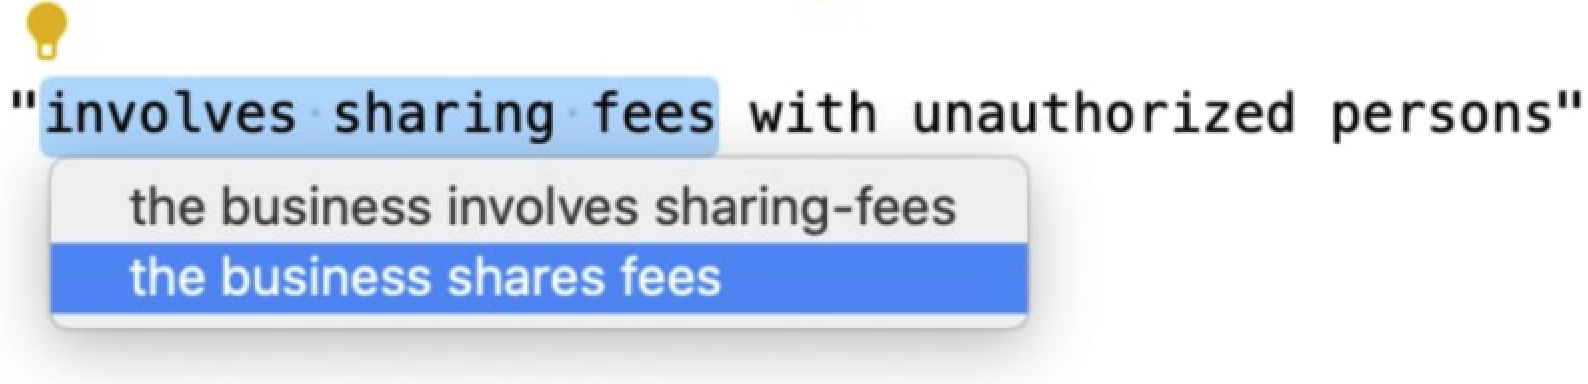
\includegraphics[width=8cm]{images/ide-mockup.png}
\caption{Future editor support (mockup)}
\label{fig:ide}
\end{figure}


\paragraph{Disambiguate adjuncts internally}
After the top-level disambiguation, we check whether the temporarily excluded adjuncts have something to disambiguate internally. 

%\begin{itemize}
%    \item \textit{involves sharing fees with a business or trade in Bali}
%\end{itemize}

%This is yet another orthogonal ambiguity, and makes the total number of trees 15. 

Suppose, for the sake of example, that the original predicate was, instead 
\textit{involves sharing fees with any business or trade in Bali}.
In such a case, we first disambiguate the internal structure of the adverbial (\textit{with any business or\dots}), using the same method as before:
apply another set of transformation functions to the adjuncts to produce disambiguation alternatives, and ask the user which one they meant.
%Adjuncts can be disambiguated with a similar set of applying the same transformation functions as to the main predicate where we had removed adjuncts, except that we don't add a subject.


Sometimes, the difference in adjuncts is linked to the difference in the main tree, in which case, we're done after picking the correct adjunct. But in our example case, the ambiguity is orthogonal to the adverbial attachment, so we need one more step.
%In any case, doing this step is not a waste of time. In the best case, solving it solves all ambiguity, and in the worst case, the ambiguity of adjunct is orthogonal to the main structural ambiguity, and solving internal adjunct ambiguity still reduces the options to show.}


\paragraph{Disambiguate adjunct attachment}
Once we have disambigated everything else---in the main tree or recursively in the subtrees---the remaining ambiguities (if any) should be related to attachment. If the user chose \textit{sharing} to be a verb, we present the following alternatives.

{\begin{enumerate}[label=\alph*)]
    \item involves with unauthorized persons 
    \item shares with unauthorized persons
    \item fees with unauthorized persons
\end{enumerate}}


 
%\end{enumerate}


%Here the user chooses option b, and 
\paragraph{Verifying the answer}
After the interactive disamgibuation, 
we show the result: \textit{involves [sharing with unauthorized persons] fees}. If the user is unhappy with the result, they may revert the disambiguation and start over.

Once a user is familiar with the precise CNL, they may write the initial description with it, and hence skip the interactive process. The IDE tries to parse the input as both variants. 


%%%% OLD VERSION OF ALGORITHM SECTION
%\paragraph{Top level disambiguation}
%At first, we apply a function which removes all postmodifier adjuncts, as shown in Table~\ref{tab:removeAdjuncts}.
%\footnote{The GF grammar makes removing adjuncts almost trivial: there are separate structures for obligatory complements that are introduced with a preposition (\textit{believe in \_}) and an optional adjunct---we simply remove the latter. The verbs \textit{share} and \textit{involve} are in the lexicon as transitive verbs with a direct object, so the only parse for \textit{with unauthorized persons} is an adjunct, not a complement.}
%We leave all obligatory complements in place, but we strip away any postmodifier adjuncts inside them, leaving only head with optional light modifiers. %Table~\ref{tab:removeAdjuncts} shows examples of this step.
%Removing adjuncts leaves us with only two different trees
%one ambiguity: whether \textit{sharing} is a noun or a verb. 

%Now, on all of the remaining trees, we apply a number of transformation functions. 

%The patterns are so specific, that it is unlikely for more than one to match a given predicate, after the adjuncts have been stripped. Figure~\ref{fig:algorithm} shows an example transformation.
%This step gives us two questions---exactly the ones we saw in Section~\ref{sec:disambiguation}). The question \textit{business involves sharing-fees} maps to the 2 trees where \textit{sharing} is a noun, and the question \textit{the business shares fees} maps to the 3 trees where \textit{sharing} is a verb.


\section{Future work}
\label{sec:futurework}

%\todo[inline]{ "The use case (computational contracts) nor an application domain (criminal activities?) is not well explained while we know that a small domain and specific use case will increase the success of adoption."

%We are planning to do a user study in a small domain -- insurance? Rule 34? We're looking for a potential use case, and once we have it, we will develop the CNL in conjunction with the use case. This will also lead to an evaluation with domain experts as subjects. -- attempted in paragraph below. Qn: Need to specify and ref rule 34?}

At present, we have worked on the CNL only inside the project, occasionally consulting an expert legal knowledge engineer, who is a part of our team.
Next steps are to find a real-life use case with a more diverse team of users and conduct an evaluation. We expect that we need to change the CNL, as it goes from our hands to the hands of non-experts. It will be interesting to see whether it also needs to change from domain to domain: aside from different lexicon, would two unrelated fields, such as insurance and construction site regulations, need any changes in the core CNL? 

%namely in the domains of insurance, a field within construction and a statute that legislates the legal practitioners (rule 34).
%The formulation process sometimes involves consultation with legal experts to arrive at an accurate interpretation of the rules. The pipeline also includes evaluations with the respective domain experts as subjects to validate that the CNL is robust enough to sufficiently and accurately describe the input and the output feedback.

In order to make L4 and the CNL easier to use, we will add editor support and robust fall-back options. We will also create a specification and resources for user guidance for the CNL, and add languages other than English.

\paragraph{IDE support} 
L4 has a plugin for Visual Studio Code, and we plan to integrate editor support for the CNL as well. 
Figure~\ref{fig:ide} shows a sketch of a potential user interaction.
We may also experiment with hovering over single words to provide information about part-of-speech, or show dependency structure---for instance, an arrow from \textit{with unauthorized persons} to all of its possible heads.


%This tool is integrated with the lexicon and conceived to give visibility to the user of all options related to a selected variant by hovering over it. The user can then select his intended option, thereby further aiding in disambiguation. With the option to select, this feature is designed to enhance informativeness for the user.

%\paragraph{Resources for user guidance} 
%Being open-sourced, the user resources will include an online repository (likely on GitHub) for easy and free access. It would contain binaries to include the necessary installation to run an example case. As such, templates for the abstract syntax, concrete syntax, CNL lexicon, binaries for the underlying GF RGL, eCASP reasoner, VSC plugin, along with a video to showcase the example and a README.txt file for instructions to execute the program will all be made available. 

\paragraph{Robust fall-back options}
\label{sec:graceful_degradation}
%We envision two stages of 
First, suppose that the natural language description is parsed in the host grammar, the GF RGL, 
but there are no transformation functions that spell out the ambiguities (as explained in Section~\ref{sec:parsing}),
nor is it covered by the precise CNL.
We will experiment with alternative methods of disambiguation, such as choosing a part of speech for individual words and showing dependency relations between words.
%the user will be able to clarify the sentence by choosing the correct parts-of-speech of individual words. 
These require more knowledge about grammar, but they work for any tree that is successfully parsed, and are thus more robust.

%In the event that unambiguous rendition of the natural language sentence fails,  The parser presents the user with all plausible definitions, and if the sentence is still ambiguous, this limits further options that the user will be presented with to syntax trees containing that specific definition, until the user is left with one unambiguous CNL sentence.
    
%Sentence fragments, including single word fragments which lack the helpful framework of context, can be disambiguated in this way.
 
Currently lexicon entries are generated from a WordNet lexicon in GF \cite{angelov2020parallel}, and a few words that we have added after finding them in the sources of our small experiments. Where a word or phrase cannot be parsed from a pre-existing lexicon, the user will be prompted to define every out-of-vocabulary word, and include it in a user-defined lexicon. We will use GF's smart paradigms \cite{detrez-ranta-2012-smart} to make an initial guess from a limited number of word forms, with a possibility to correct any wrong guesses.
%, which will hopefully enable this disambiguation engine to be useful in different languages and with specialized vocabularies.

In the case that parsing still fails, the sentence is syntactically out of scope from the CNL. Already now, the parser could try to break the sentence down into phrases that can be parsed, but we would need to guide the user how to reconstruct the whole sentence to be within the scope.
We recognize the limits of the GF parser in handling ungrammatical output, and may look into more robust parsing pipelines, such as dependency trees to GF abstract syntax \cite{kolachina2016abstract}.

%A possible solution is for the parser to split the sentence by delimiters like spaces or dashes into separate words, and clarify each ambiguous word individually by user input. For example, the phrase (\textit{all mimsy were the borogroves}) contains nonsensical words and cannot be parsed. The parser would then prompt the user for the definitions of (\textit{mimsy}) and (\textit{borogroves}).

%\paragraph{Specification of the CNL}
%So far the CNL itself is a prototype, and we may add or remove features as we see fit. As the CNL matures, we will write a specification as an authoring guide---this will also help the user to write grammatical sentences.

%\paragraph{Alternative disambiguation methods}
%However, ideally the parser would be able to assume that a word in between a determiner and verb is a noun, or that a single word that follows an article is a noun. We plan to look into non-GF-based 

%If even this fails, the parser would ideally throw up an error and ask the user to rephrase the sentence in a CNL way, or possibly break the sentence down into phrases that can be parsed.



\paragraph{Multilingual support}

So far, we support the translation of L4 to English, with a view to support multiple languages in the near future. 
With multilingual output, we need to also support word sense disambiguation and multi-word expressions. For instance, a term like \textit{sole proprietor} will be wrong in many languages, if translated compositionally: ``lonely proprietor'' instead of the correct multi-word term. As we work on a use case in a specific domain, it will be more realistic to have a good coverage for a lexicon.

As for word sense disambiguation, our short-term plan is to use WordNet \cite{fellbaum1998wordnet} glosses to ask the correct sense for each word. Longer-term, we may look into statistical methods for guessing the most likely word senses.

%Our current method distinguishes a term like \textit{sole proprietor} from the hypothetical compound noun \textit{sole-proprietor}, but even with the correct part of speech for \textit{sole}, a compositional translation will be wrong in many other languages.
%, resulting in something like ``lonely propietor''.

%As 

%Currently, our implementation targets only English, as both source and target. However, given GF's support for multilinguality, we extending to other languages is just a matter of more engineering.


%The interface would also be made more user friendly by providing an autocorrect function that suggests words present in the lexicon or previously-used terms, as well as drop-down lists for users to select autocompleted words and disambiguate definitions. Numbers, which are currently parsed as strings, would be parsed as integers, and there would be verification of specific inputs such as email addresses.

%Successful parsing would generate a consolidated summary for confirmation, with an edit function for the user to edit any input errors. There would also be an option to forward the output to multiple platforms and formats (eg. email, a generated pdf).

%TODO: picture of dependency parsing? Future work: show this visually

% Option:
% Ask about the head of the subtrees as a way of asking for attachment
% E.g.
% b) involves sharing, sharing fees
% c)  , fees with persons

%As future work, we expect to  providing word senses, with the help of WordNet~\cite{fellbaum1998wordnet}.

%As the work matures, each of these there subtasks could become a full paper in itself. However, we are not there yet---as of April 2021, there are prototypes of all the parts, but not yet a full working pipeline combining all. 
%In this paper, we present on a high level the full system, and in more detail, some interesting solutions we've developed in the course of the project.

%

%\texttt{Jaywalk} or \texttt{Criminal}, such as the example below.

%\begin{verbatim}
%InvolvesPaymentOfCommissions-
%ForLegalWorkByUnauthorizedPersons-
%PerformedByTheLegalPractioner
%\end{verbatim}


%\section{Word sense disambiguation}
%\label{sec:lexicon}

%Word sense disambiguation is mostly subconsciously interpreted by humans, where meaning is derived from context. Word sense disambiguation wasn't important when considering monolingual use, but is important if the parser will be useful in multilingual settings. We use WordNet \cite{fellbaum1998wordnet} for our current lexicon, and glosses. 

%Where lexicon mapping doesn't exist, or it's not found on WordNet, currently we are just generating a GF lexicon entry with a smart paradigm \cite{detrez-ranta-2012-smart}.

%\noindent Currently, we offer two alternatives.

%\paragraph{Based on name} We can parse the name, infer the valency from type signature, and ask clarification, if necessary. For instance, \texttt{is\_associated\_with : Business -> Business -> Bool} is a transitive verb phrase.

%Where there is ambiguity, we can ask the user to clarify which part of speech the word belongs to. For example, \textit{criminal} could be a noun or an adjective.

%We can then ask the user to narrow the meaning by choosing the WordNet synset. Here, if the user chooses \textit{criminal (adjective)}, this has several senses in WordNet, which are inherited in the GF-WordNet lexicon. The user can then specify if they mean \textit{criminal} as in \textit{condemnable}, \textit{guilty of crime or serious offense}, or \textit{felonious}.


%\paragraph{Based on description} A description can also be assigned to a predicate for disambiguation in a user-defined lexicon. \textit{Criminal} can be mapped to a longer string:  \textit{"pertaining to or involving a crime"}. The predicate name is used in the body of the contract, but the NLG engine will use the description.

%\paragraph{POS given explicitly} The WordNet POS tags can be set explicitly in the user-defined lexicon. For example, if we want \textit{criminal} to have the meaning of \textit{felonious, having the nature of a crime}, so we would define it in the lexicon as \begin{verbatim}Criminal -> criminal_3_A\end{verbatim}.

%\textit{person} has many senses in WordNet \cite{fellbaum1998wordnet}, and those senses are inherited in the GF-WordNet lexicon, so we must specify that we mean \textit{person} as in human being, rather than a grammatical category ("3rd person singular").


%\paragraph{Based on description} A predicate like \texttt{UnauthorizedSharingFees} is mapped to a longer string:  \textit{"involves sharing fees with unauthojurized persons for legal work"}. The predicate name is used in the body of the contract, but the NLG engine will use the description.
%\end{itemize}

%\paragraph{POS given explicitly}

%\subsection{Parsing the user-defined predicates}


%include a lexicon. Currently, the lexicon entries are just words from the GF-WordNet \cite{angelov2020parallel} lexicon, but in the future, we will support other sources, including user-defined lexicon, and methods which don't rely on inputting arbitrary numbers.

%\begin{verbatim}
%lexicon
%
%Person -> person_1_N
%Jaywalk -> jaywalk_V 
%Criminal -> criminal_N
%\end{verbatim}




%EVERYONE: write here whatever you like

%\begin{itemize}
%    \item Multiple languages
%    \item autocorrect interface
%    \item interface to drop/select -> esp drop/select wn definitions
%    \item validity check of particulars (e.g valid email address, postal address), integers instead of strings for amount
%    \item discrepancy check of details e.g sharing fees amounts of zero amount
%    \item definition/explanation that goes with technical terms in the questions
%    \item open-ended box lastly for important details ?
%    \item a consolidated summary that aggregate all the inputs as a summary for confirmation with edit function to amend any earlier input.
%    \item options to fwd generated output to multiple platform (email, whatsapp etc)
%    \item maybe parts of speech can eventually be inferred from sentence structure?
    
%\end{itemize}




\section*{Acknowledgements}

This research is supported by the National Research Foundation (NRF), Singapore, under its Industry Alignment Fund --- Pre-Positioning Programme, as the Research Programme in Computational Law. Any opinions, findings and conclusions or recommendations expressed in this material are those of the author(s) and do not reflect the views of National Research Foundation, Singapore.

% Entries for the entire Anthology, followed by custom entries
\bibliography{bibliography}
\bibliographystyle{acl_natbib}


\end{document}
